% Q17 -- BIST / BILBO system block diagram: PRSG -> Logic Cloud -> Signature Analyzer (MISR);
% syndrome shifted out via the scan chain. Mode select C[1:0] table included.
\documentclass[border=10pt]{standalone}
\usepackage{tikz}
\usetikzlibrary{arrows.meta,positioning}
\begin{document}
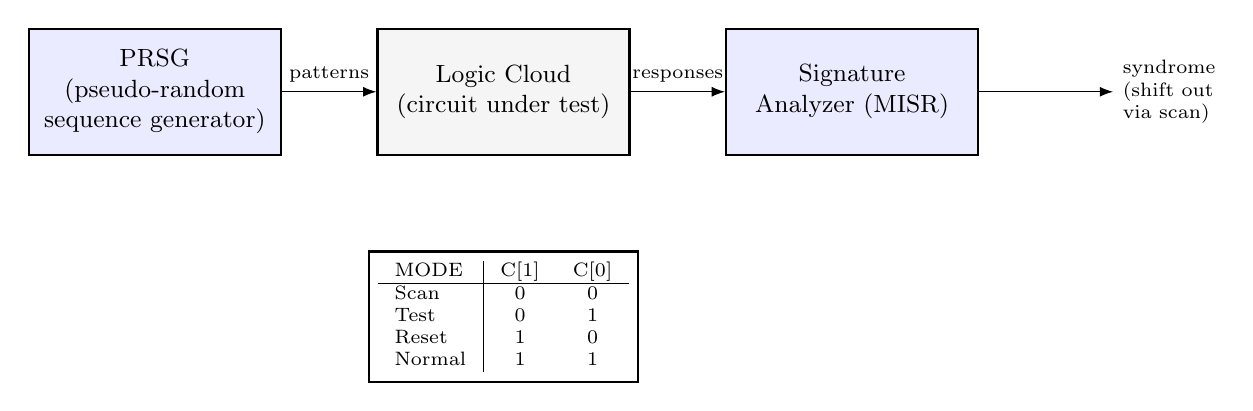
\begin{tikzpicture}[>=Latex, font=\small,
  box/.style={draw, thick, minimum width=3.2cm, minimum height=1.6cm, align=center}]
\node[box, fill=blue!8] (prsg) {PRSG\\(pseudo-random\\ sequence generator)};
\node[box, fill=gray!8, right=1.2cm of prsg] (cloud) {Logic Cloud\\(circuit under test)};
\node[box, fill=blue!8, right=1.2cm of cloud] (sig) {Signature\\ Analyzer (MISR)};
\draw[->] (prsg) -- (cloud) node[midway,above,font=\scriptsize]{patterns};
\draw[->] (cloud) -- (sig) node[midway,above,font=\scriptsize]{responses};
\draw[->] (sig.east) -- ++(1.7,0) node[right, align=left, font=\scriptsize]{syndrome\\(shift out\\ via scan)};
% mode table
\node[draw, thick, below=1.2cm of cloud, font=\scriptsize] (tab)
 {\begin{tabular}{l|cc}
   MODE & C[1] & C[0]\\ \hline
   Scan   & 0 & 0\\
   Test   & 0 & 1\\
   Reset  & 1 & 0\\
   Normal & 1 & 1\\
  \end{tabular}};
\end{tikzpicture}
\end{document}
